\chapter{Long Term Evolution for Railways (LTE-R)}
\label{chapter4}

\section{LTE-R Communication System}
LTE-R System Description To provide improved and more efficient transmission for
HSR communications, it is vital to consider frequency and spectrum usage for LTE-R. HSRs are important stra-
tegic infrastructure, and, in some countries, this argument is being leveraged to convince governments that
large spectrum chunks need to be allocated specifically for it. Some industry bodies, including the European
Railway Agency (ERA), China Railway, and UIC, are working to secure spectrum allocation for HSR use. Currently,
most LTE systems work at the bands above 1 GHz, such as 1.8, 2.1, 2.3, and 2.6 GHz, although 700–900-MHz
bands are also used in some countries. Large bandwidth is available in the upper bands, giving a higher data rate,
whereas lower frequency bands offer longer distance coverage. Figure 1(b) summarizes the possible frequen-
cy bands for LTE-R in China, Europe, and Korea. As a high-frequency band has larger propagation loss and
more severe fading, the radius of an LTE-R cell would be <2 km [due to the strict requirement of signal-to-noise ratio (SNR) 
and BER in HSR], leading to frequent handovers and a requirement of substantial investment for higher BS density. Therefore, the low-frequency bands,
such as 450–470 MHz, 800 MHz, and 1.4 GHz, have been widely considered. The 450–470-MHz band is already
well adopted by the railway industry; therefore, dedicated bandwidth for professional use can still be allocated
from local regulators. Furthermore, the carrier aggregation capability of LTE will permit the use of different bands to overcome problems of capacity. Figure 1(b)
presents the detailed frequency allocation of 450 – 470  MHz in China [12], and it is feasible to allocate
enough bandwidth for LTE-R within this band. In Europe, the FRMCS of UIC would like to build on the current GSM-R investment by reusing the existing mast
sites, which could save as much as 80–90\% of the cost of a network. Railways are also concerned about continu-
ing to make use of their GSM-R masts, and, therefore, a spectrum allocation under 1 GHz is more cost effective
in Europe. However, the selection of frequency band depends on government policy and differs by country.
\begin{figure*}[t]
\label{fig:ltearch}
\centering
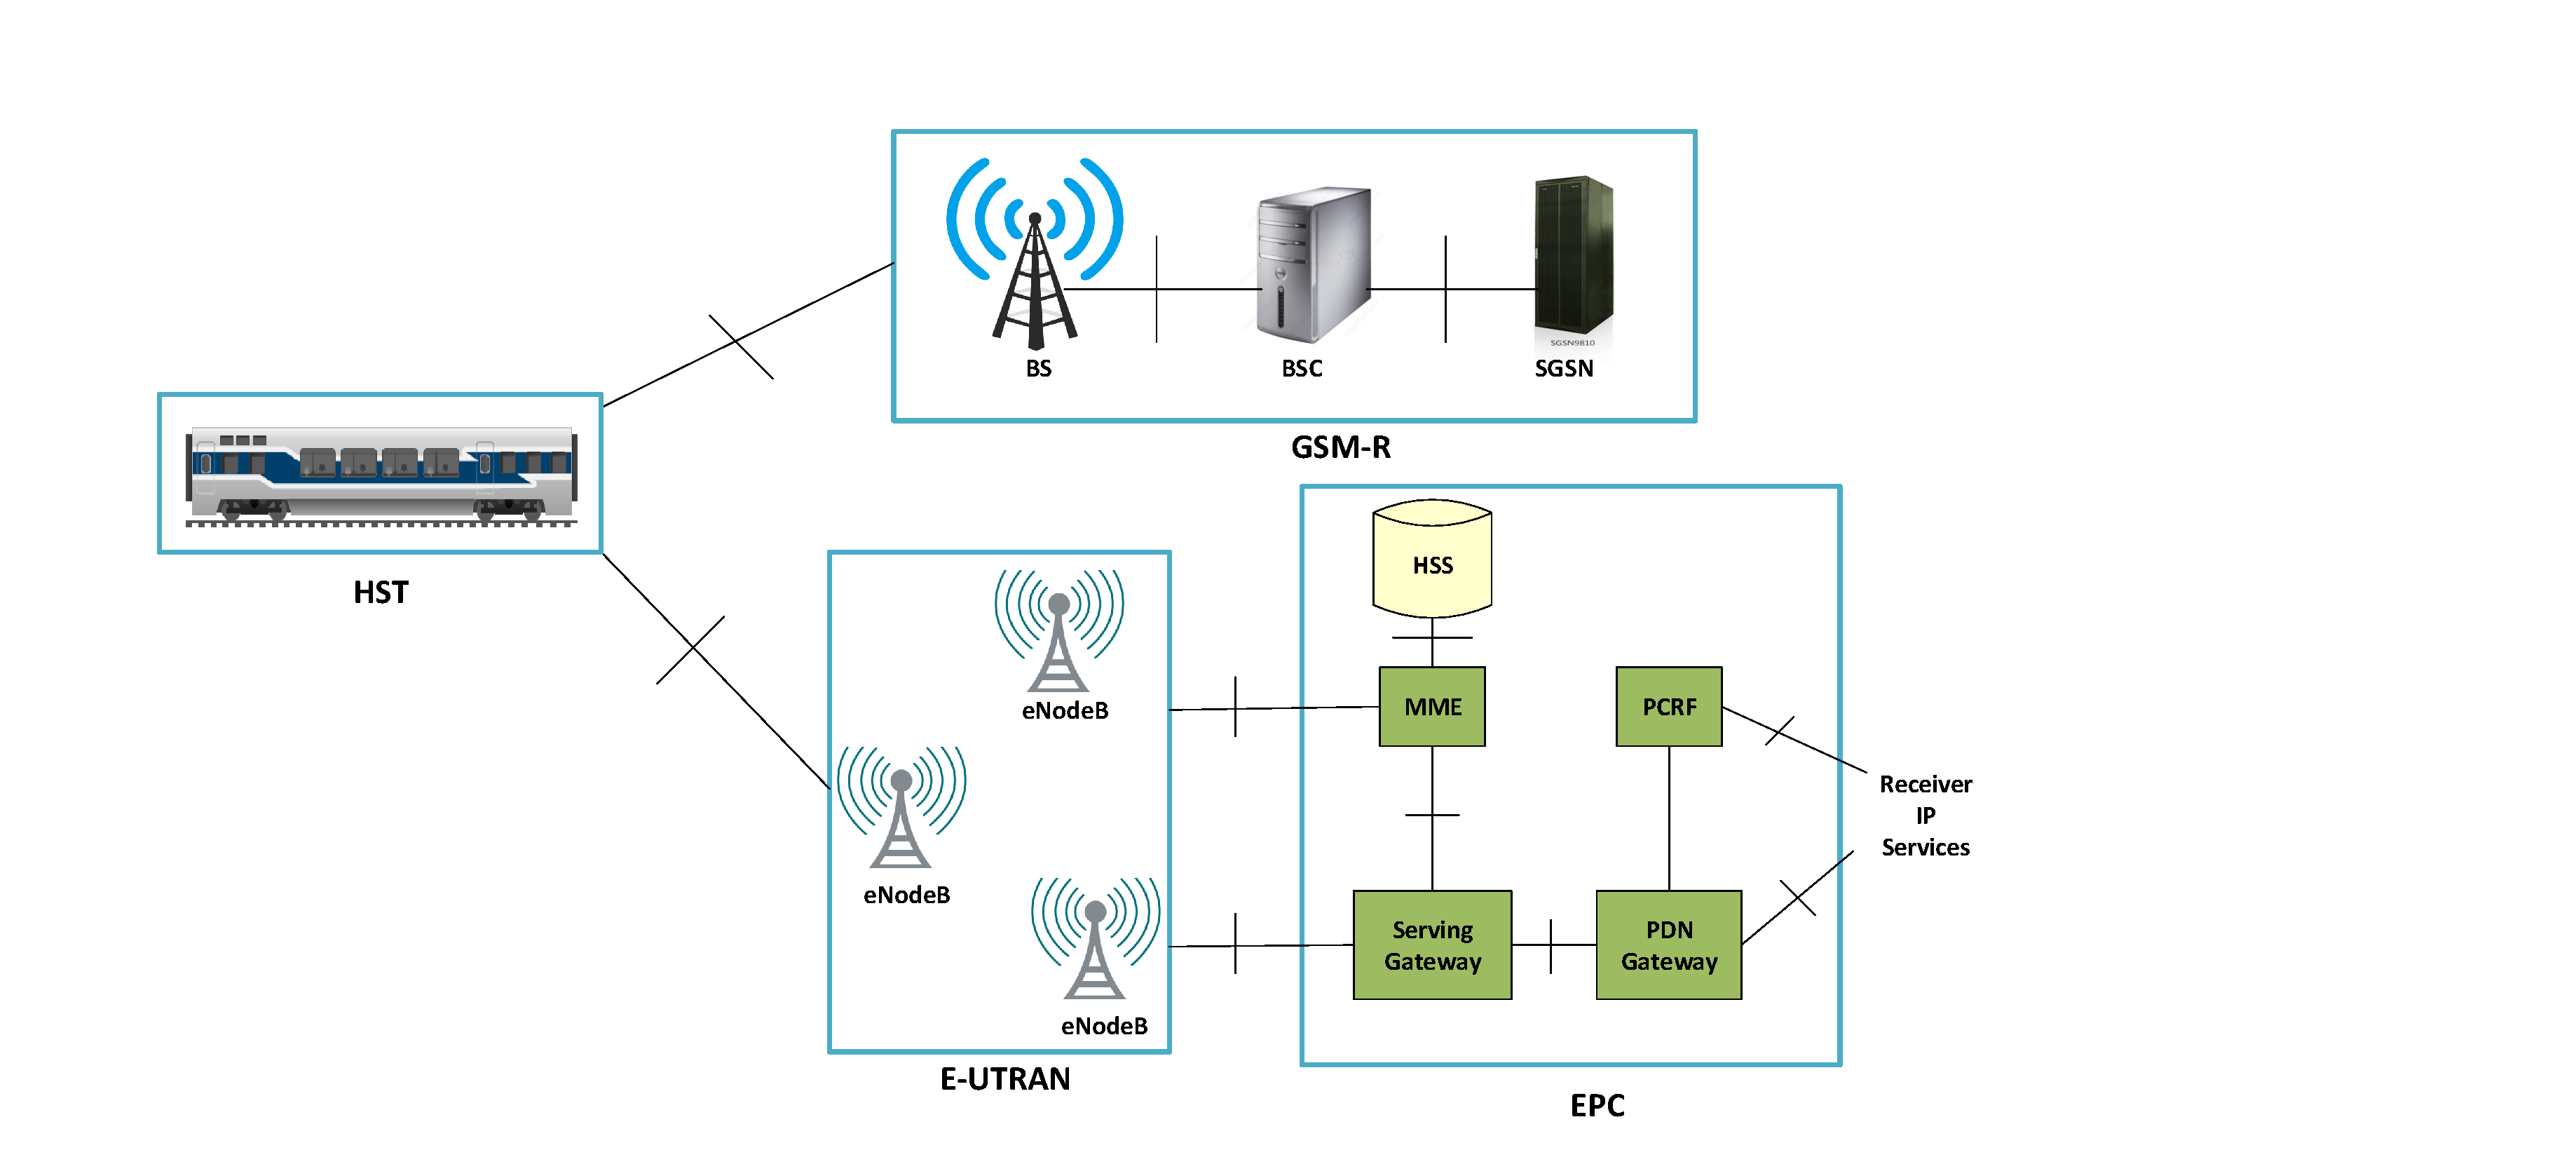
\includegraphics[width=\linewidth,keepaspectratio]{images/Gill/lte_figs/lter_architecture.eps} 
\caption{High speed train inside a tunnel for LTE-R. $D_{LOS}$ is the distance between transmitter and receiver, $d$ is the distance between the LCX cable transmission slots.}
\end{figure*}


Standard LTE includes a core network of evolved packet core (EPC) and a radio access network of Evolved
Universal Terrestrial Radio Access Network (E-UTRAN). The Internet protocol (IP)-based EPC supports seamless
handovers for both voice and data to cell towers, and each E-UTRAN cell will support high data and voice capacity by
high-speed packet access (HSPA). As a candidate for the next-generation communication system of HSR, LTE-R in-
herits all the important features of LTE and provides an extra radio access system to exchange wireless signals with
onboard units (OBUs) and to match HSR-specific needs. The future architecture of LTE-R according to [4] is pre-
sented in Figure 2, and it shows that the core network of LTE-R is backward compatible with GSM-R.

Compared with the public LTE networks, LTE-R has many differences, such as architecture, system parameters, network layout, services, and QoS. The preferred
parameters of LTE-R are summarized in Table 1, based on the future QoS requirements of HSR communications. Note that LTE-R will be configured for reliability
more than capacity. The network must be able to operate at 500 km/h in complex railway environments. Therefore, quadrature phase-shift keying (QPSK) modulation 
is ­preferred, and the packet number of retransmission must be reduced as much as possible.[RuisiHeBoAiGongpuWang/HSRCommunications]


\section{Leaky Coaxial Cable}
Substantial work has been done for the radio communication in tunnel environments. 

\begin{figure}[!ht]
\label{fig:leakcoax}
\centering
\includegraphics[width=\linewidth,keepaspectratio]{images/Gill/lte_figs/leakycoax.eps} 
\caption{Leaky Coaxial Cable}
\end{figure}

Authors of [2]measure the radio channel frequency response; the large scale and small scale
fading in tunnel are investigated through field experiments. Statistical characteristics of the propagation channels are
suggested in [3]. Both [2] and [3] indicate that WLAN cannot achieve good performance when used in tunnel environments.
As a result, leaky waveguide and leaky coaxial cable are used in wireless communication due to their stability and
robustness from the interference. The availability of train ground communication in subway systems by waveguide is
analyzed in [4] and [5]. Meanwhile, leaky coaxial cable is lso studied. H. Cao [7] introduces the way to calculate frequency range of LCX and shows experimental results about
LCX performance at 1.8GHz. Authors of [11] introduce the propagation at 2GHz in an enclosed area using a leaky coaxial
cable. Authors of [12] study the theory of leaky coaxial cable with periodic slots, and frequency band of the studied LCXs
is from 450MHz to 900MHz. However, few people specialize in the performance of leaky coaxial cable at 2.4GHz band, especially the application in tunnels.[HongweiWangBinNingandHailinJiang]

\section{Channel Impairements Inside a Tunnel}
The tunnel environment is affected by multipath and diffraction effects due to multiple reflections from the tunnel walls,
which leads to a substantial fading environment. By deploying LCX cables, we can eliminate the large penetration loss
due to tunnel walls. However, small-scale fading can still cause a large amount of errors and decrease the QoS for the communication link.

High velocity trains experience very high Doppler shifts and a fast fading channel. These problems can lead to significant
BER degradation of the LTE system. The frequency shifts caused by the Doppler phenomenon can lead to shifts in the
sub-carrier frequencies for OFDM, which leads to synchronization errors. The maximum Doppler shifts for a train traveling at 500 km/h is 2.314 kHz for a 5 GHz carrier frequency.
This large Doppler shift can also lead to significant drops in the quality of wireless signals and increase the bit error rate. Thus,
to develop an efficient and reliable communication link inside tunnels, we need to properly model this channel impairment
and build our proposed channel model by taking into account these tunnel phenomenons. These impairments are described in detail in the following subsections.[OwnPaper]

\subsection{Multipath Fading}
The following time-varying multipath channel impulse response considers the effects of Doppler shift and scattering [11]: where τ is the path delay, t is time in seconds, δ[τ − τ k (t)]
is the impulse response, f c is the carrier frequency, h k (t) is the envelope of the time-varying channel and consists of both
large and small-scale fading components. Since the structure of LCX is almost the same as a leaky waveguide, the large
scale fading of channel can be modeled linearly [8]. There is also no signal shadowing and the line-of-sight (LOS) signal
component is always present along the tunnel. This type of channel fading can be best described by a Ricean fading
model. The probability density function p(α) of a Rician fading model is given by [10]: where K is the Rician factor and α is the complex amplitude of
the channel response function that has a unity second moment. 

\subsection{Doppler Shift}
The 3GPP channel model [14] is used for its Doppler shift profile in high speed railway environment. The measurements
obtained for the Doppler frequency shift are implemented for two scenarios. The first scenario is for an open space while
the second scenario is for high speed trains. Doppler shift is not taken into consideration. There exists a third scenario for
tunnels using multiple antennas. Since the slots of LCX can be modeled as multiple antenna system, we use this Doppler shift
profile for our proposed channel. The Doppler shift variation f s (t) is described by

\begin{figure}[!ht]
\label{doppler}
\centering
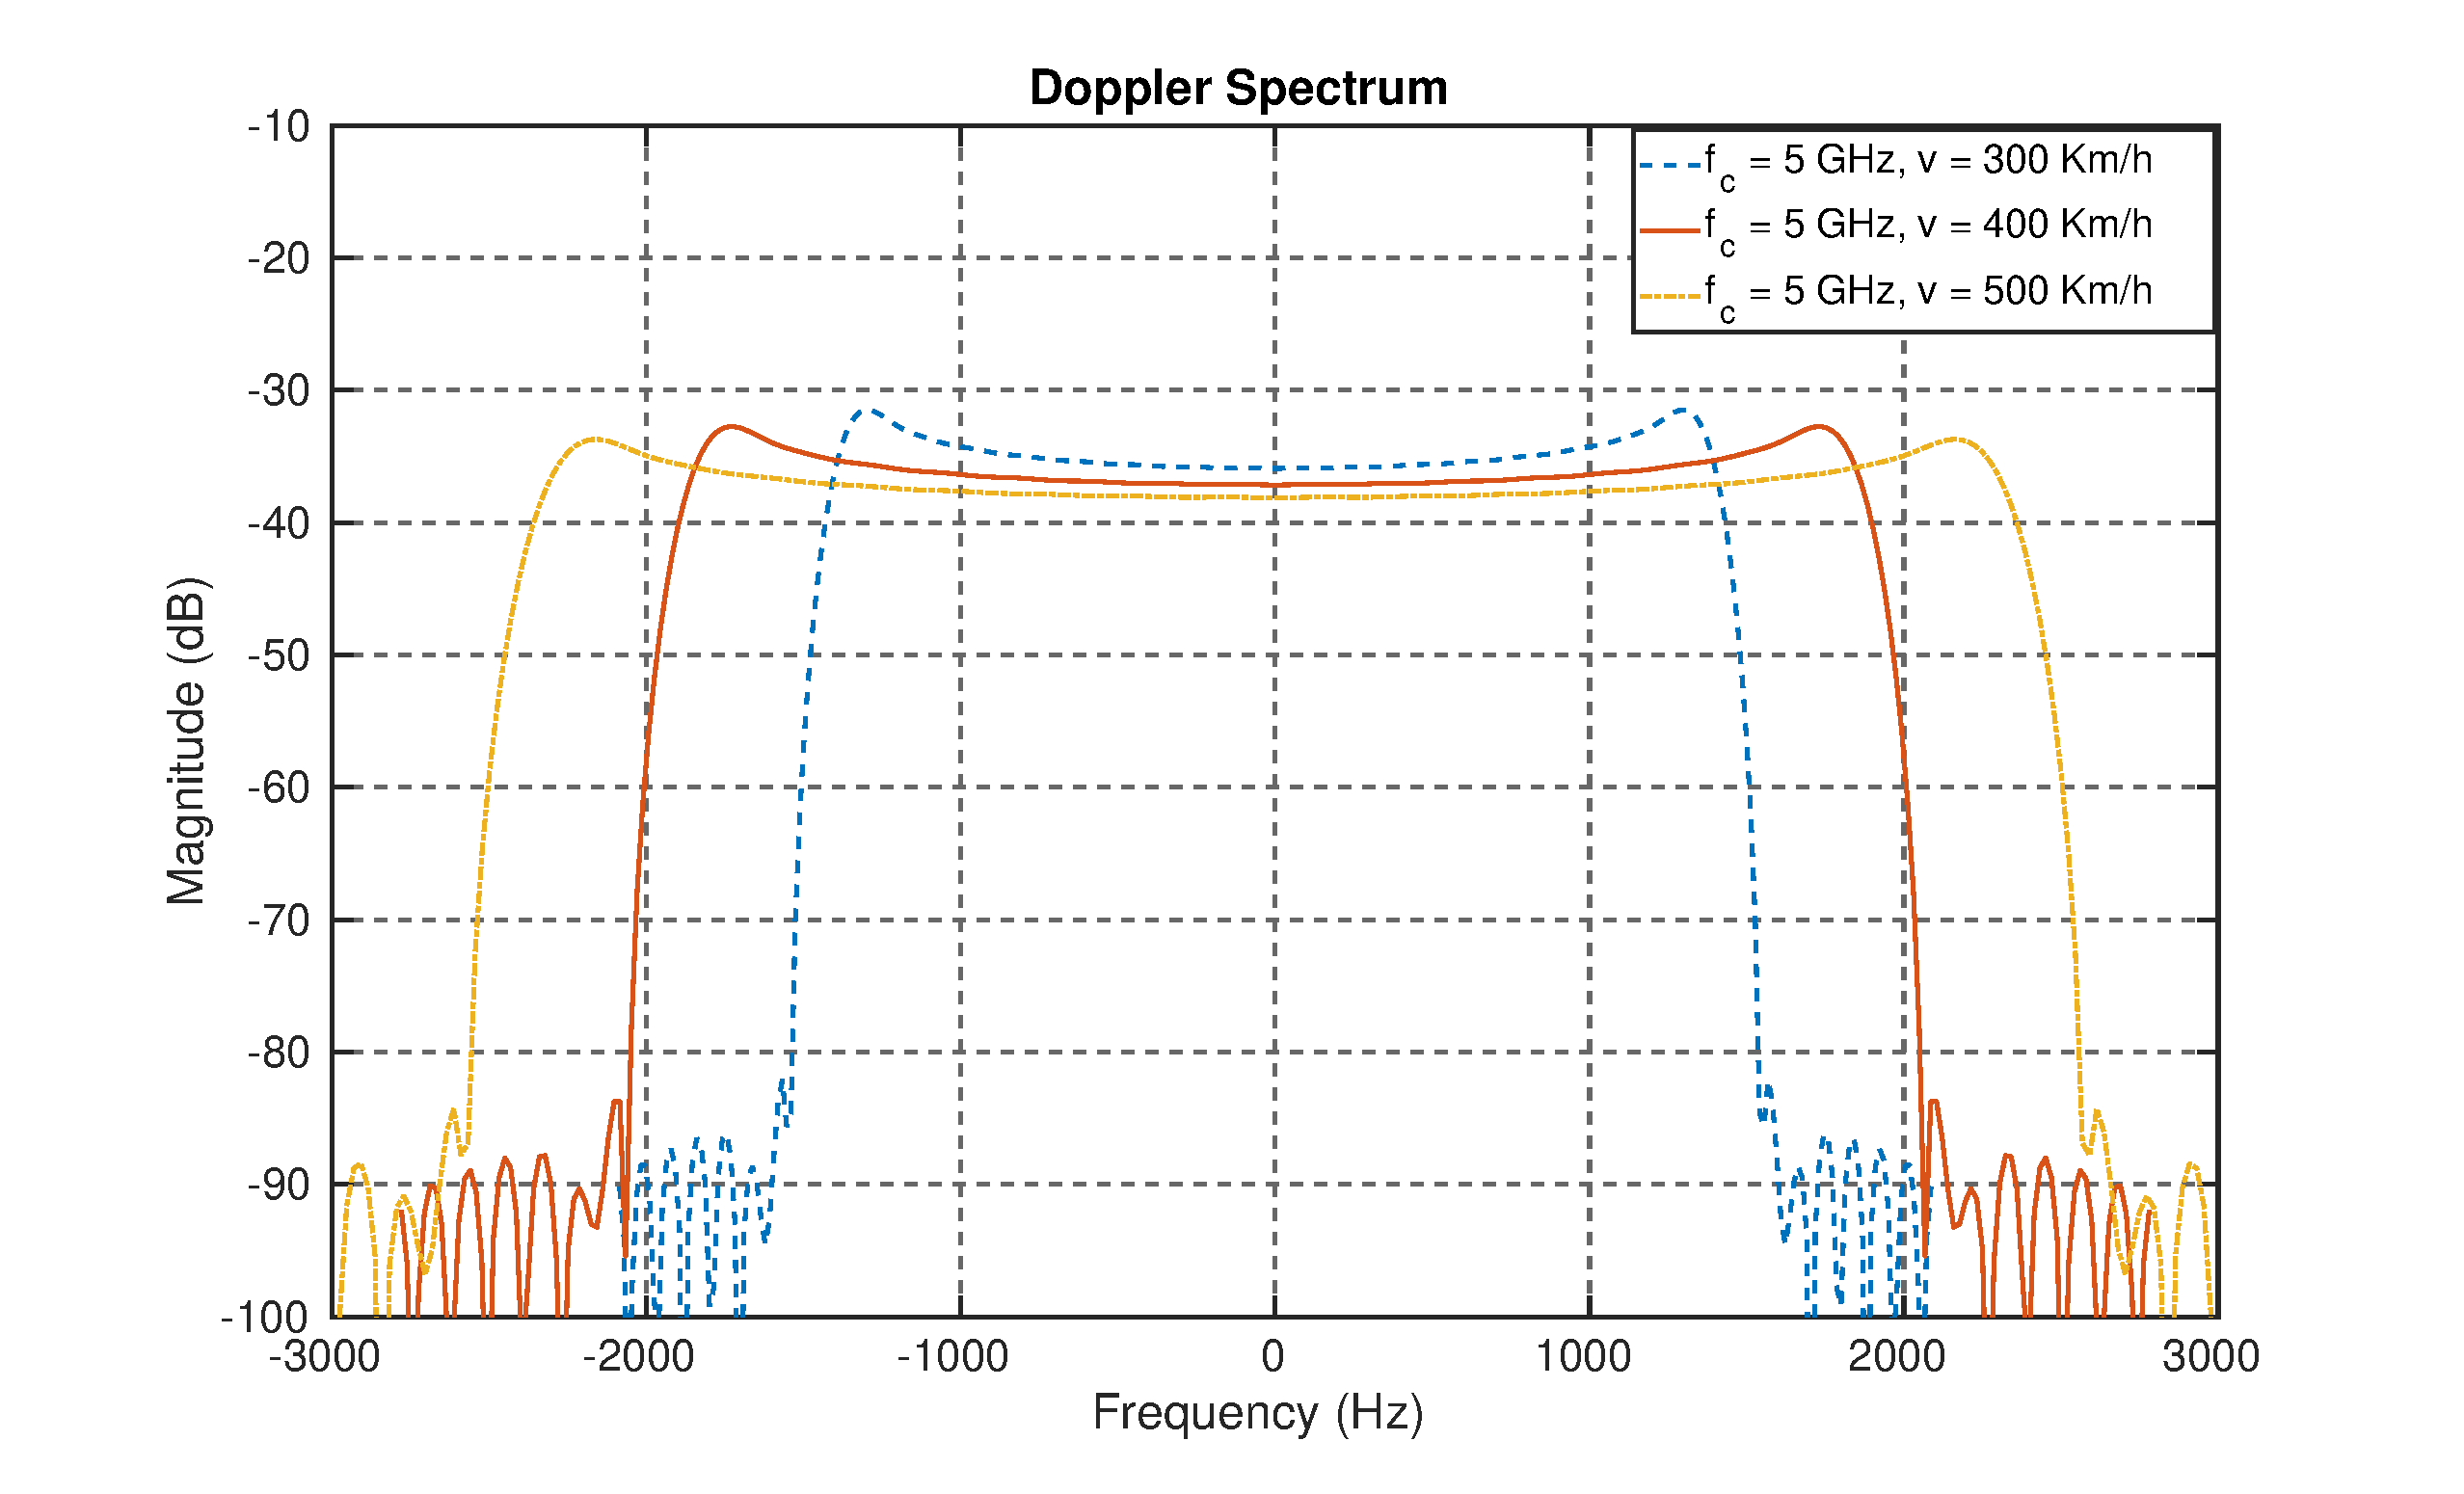
\includegraphics[width=\linewidth,keepaspectratio]{images/Gill/lte_figs/dopplerspectrum.eps} 
\caption{Doppler spectrum for LTE-R at different train velocities $v$ (km/h) = 300, 400 and 500 and $f_c$ = 5 GHz.}
\end{figure}

\section{Two-Ray Propagation Model}

\subsection{Classical Two-Ray Propagation Model}



\subsection{Dynamic K-factor}

\section{Summary}
This chapter outlined and examined the topics of jamming and anti-jamming techniques, and provided a foundation in communication system theory and advanced equalizer design.  Secondly it setup an understanding of Software-Defined Radio, the power of such an architecture, and examples of implementations and existing software for future designs.  Next, this thesis will consider a new anti-jamming technique and design an implementation of such a system.  After the implementation is investigated, the result of specific experiments on such an implementation will be analyzed.\\
